\section{Functional Robustness and Query Horizon}
\label{sec:functional}

\subsection{Retrieval under controlled damage}
\label{retrieval-under-controlled-damage}

We evaluated retrieval on the 5,000-node PrimeKG subgraph using the fixed
benchmark from Section~\ref{sec:data}. The benchmark contains 200
drug--disease pairs that were retrievable in two hops before damage. One hundred had one such path, and one hundred had multiple paths. We used the same
queries and group assignments at every damage level. If a drug or
disease was removed, its query counted as a failure and remained in
the denominator.

For each damaged graph, the retriever builds sets of the surviving
protein neighbors of each drug and disease. A two-hop query succeeds
when those sets intersect. The size of the intersection is the number
of surviving two-hop paths. For larger hop limits, the retriever
computes the shortest unweighted distance $d_{\mathrm{PPI}}$ between
the two neighbor sets along surviving protein--protein interaction
(PPI) edges. A shared protein gives $d_{\mathrm{PPI}}=0$. If either set
is empty or no connecting PPI path exists, the distance is infinite.
The shortest allowed drug--disease path therefore has length
$2+d_{\mathrm{PPI}}$, including one edge at each endpoint. For a
finite hop limit $L$, a query succeeds when this length is at most
$L$. For unlimited hops, a query succeeds when the distance is finite.
We write $R_L(f)$ for the fraction of benchmark queries that succeed
at removal fraction $f$ and hop limit $L$.

The two-hop experiments used ten seeds (0--9) for each random removal
strategy and one fixed order each for degree- and betweenness-targeted
node removal. The hop scan used random edge removal with the same
three seeds (0--2) for $L=2,3,4,\infty$. Matching the queries and the
damage states across hop limits isolates the effect of changing $L$.

\subsection{Connectivity and retrieval under damage}
\label{connectivity-and-retrieval-separate}

At 50\% random edge removal, the largest connected component still
contained 98.2\% of the original nodes, whereas two-hop retrieval
succeeded for 43.3\% of the benchmark queries. The gap was 54.9
percentage points across the same ten damage seeds
(Figure~\ref{fig:ws3-structure-vs-retrieval}). Protein--protein edges
can keep much of the graph connected even after a query has lost its
last shared-protein route. The largest-component fraction $S(f)$ can
therefore remain high while $R_2(f)$ declines.

\begin{figure}[!htbp]
  \centering
  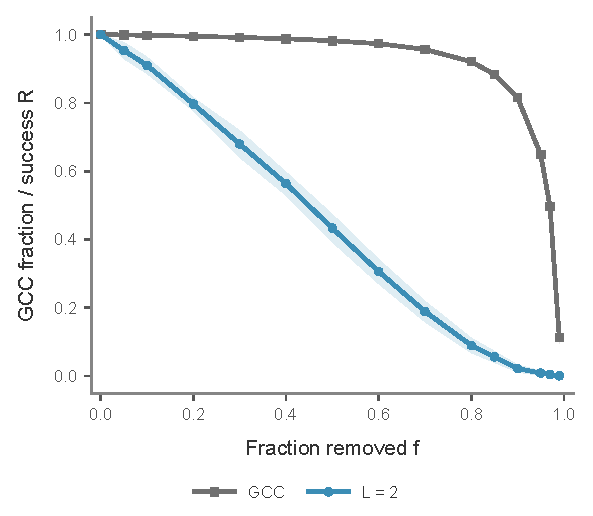
\includegraphics[width=0.88\linewidth]{act2/primekg_5000_bfs_v1/fig_S_vs_R.pdf}
  \caption{Largest connected component fraction $S(f)$ and two-hop retrieval success $R(f)$ under random edge removal. Curves are means across ten seeds. Shading shows one sample standard deviation on either side of the mean.}
  \label{fig:ws3-structure-vs-retrieval}
\end{figure}

Deleting nodes removes their incident edges and can also remove the
query endpoints themselves. At 50\% node removal, mean two-hop success
was 15.55\% under random deletion. It fell to 0\% under the fixed
degree ranking and 0.5\% under the fixed betweenness ranking. These
two targeted results describe individual deletion orders.

\subsection{Path redundancy and two-hop survival}
\label{backup-paths-and-hop-limits}

At 50\% random edge removal, two-hop success was 60.7\% for queries
with multiple original paths and 25.9\% for queries with one original
path (Figure~\ref{fig:ws3-path-redundancy}). The groups are defined by
their intact-graph path counts. A query with multiple paths remains
retrievable as long as both edges of any one of its original
shared-protein routes survive.

Under independent edge retention with probability $p$, each two-hop
path survives with probability $p^2$. Routes through distinct shared
proteins use distinct edges, so a query with $m$ such routes has
survival probability $1-(1-p^2)^m$. We used this model as a benchmark
for the fixed-count deletion experiments, averaging the predicted
probabilities over the queries in each group. On the 5,000-node graph,
the largest absolute differences between observed and predicted
group means across the tested fractions were 2.10 percentage points for
single-path queries and 3.25 for multi-path queries. The single-path
group on the 2,000-node development graph showed a larger maximum
deviation of 9.05 percentage points. The retriever agreed with an
independent NetworkX implementation on the checked development cases.

\begin{figure}[!htbp]
  \centering
  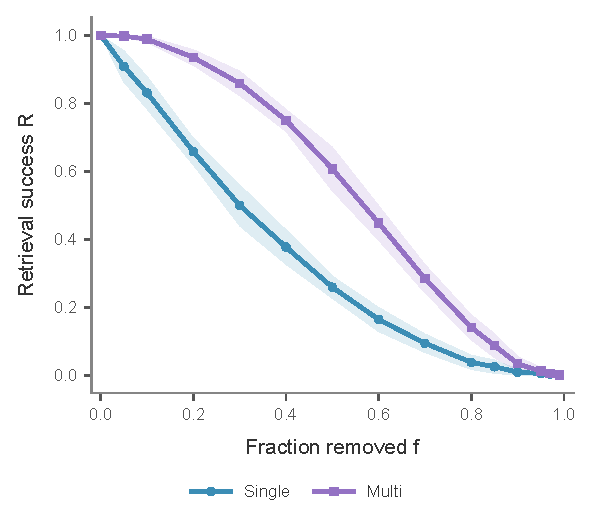
\includegraphics[width=0.88\linewidth]{act2/primekg_5000_bfs_v1/fig_R_by_group.pdf}
  \caption{Two-hop retrieval success under random edge removal, grouped by whether a query had one or multiple two-hop paths before damage. Curves are means across ten seeds. Shading shows one sample standard deviation on either side of the mean.}
  \label{fig:ws3-path-redundancy}
\end{figure}

\subsection{Effect of the hop limit}

In the matched three-seed comparison, allowing one additional PPI
step at 50\% edge removal increased mean retrieval success from
40.3\% at $L=2$ to 84.5\% at $L=3$. The mean reached 89.5\% at $L=4$
and stayed at 89.5\% with unlimited hops. The two-hop value here is
the baseline for the three scan seeds. The 43.3\% reported above is
the mean over all ten seeds.

At 90\% edge removal, the corresponding success rates were 2.0\%,
10.0\%, 28.7\%, and 37.0\%. At this higher damage level, the
8.3-percentage-point gap between four hops and unlimited hops shows
that some surviving routes require more than two PPI steps.
Figures~\ref{fig:ws3-hop-curves} and~\ref{fig:ws3-hop-heatmap} show how
success varies with the removal fraction and the hop limit. The
results describe typed path availability for an initially retrievable,
redundancy-balanced benchmark on a BFS-sampled subgraph. The measured
rates depend on both the benchmark and the allowed path length.

\begin{figure}[!htbp]
  \centering
  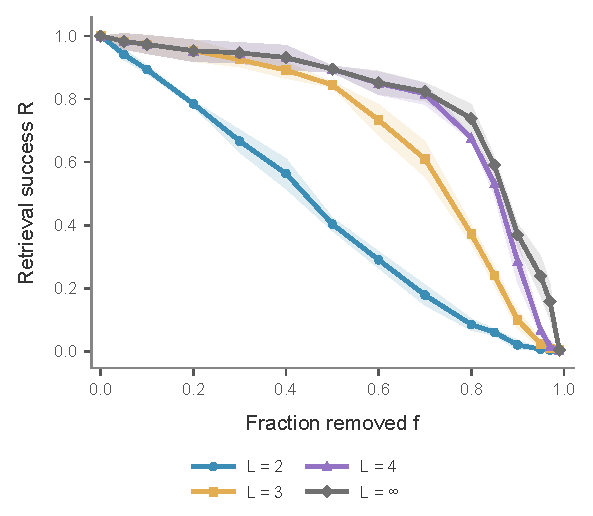
\includegraphics[width=0.88\linewidth]{act2/primekg_5000_bfs_v1/fig_R_L_curves.pdf}
  \caption{Retrieval success under random edge removal for hop limits $L=2,3,4,\infty$. All curves use the same three removal seeds. Shading shows one sample standard deviation on either side of the mean.}
  \label{fig:ws3-hop-curves}
\end{figure}

\begin{figure}[!htbp]
  \centering
  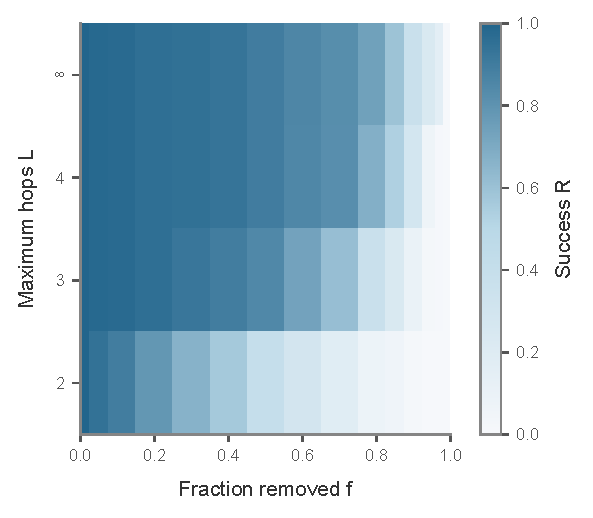
\includegraphics[width=0.88\linewidth]{act2/primekg_5000_bfs_v1/fig_R_L_heatmap.pdf}
  \caption{Mean retrieval success by edge removal fraction $f$ and hop limit $L$. Each cell averages the same three random edge removal seeds used in Figure~\ref{fig:ws3-hop-curves}.}
  \label{fig:ws3-hop-heatmap}
\end{figure}

We ran the retrieval experiments with \texttt{src/run\_ws3.py},
saved the results in \texttt{results/ws3}, and generated the four
figures with \texttt{src/plot\_ws3.py}.
